%!TEX program = xelatex
%!TEX root = ../../theory.tex

\documentclass[a4paper, openany, oneside]{memoir}
\usepackage[no-math]{fontspec}
\usepackage{pgfplots}
\pgfplotsset{compat=newest}
\usepackage{commath}
\usepackage{mathtools}
\usepackage{amssymb}
\usepackage{amsthm}
\usepackage{booktabs}
\usepackage{mathtools}
\usepackage{xcolor}
\usepackage[separate-uncertainty=true, per-mode=symbol]{siunitx}
\usepackage[noabbrev, capitalize]{cleveref}
\usepackage{listings}
\usepackage[american inductor, european resistor]{circuitikz}
\usepackage{amsmath}
\usepackage{amsfonts}
\usepackage{ifxetex}
\usepackage[dutch,english]{babel}
\usepackage[backend=bibtexu,texencoding=utf8,bibencoding=utf8,style=ieee,sortlocale=en_GB,language=auto]{biblatex}
\usepackage[strict,autostyle]{csquotes}
\usepackage{parskip}
\usepackage{import}
\usepackage{standalone}
\usepackage{hyperref}
%\usepackage[toc,title,titletoc]{appendix}

\ifxetex{} % Fonts laden in het geval dat je met Xetex compiled
    \usepackage{fontspec}
    \defaultfontfeatures{Ligatures=TeX} % To support LaTeX quoting style
    \setromanfont{Palatino Linotype} % Tover ergens in Font mapje in root.
    \setmonofont{Source Code Pro}
\else % Terug val in standaard pdflatex tool chain. Geen ondersteuning voor OTT fonts
    \usepackage[T1]{fontenc}
    \usepackage[utf8]{inputenc}
\fi
\newcommand{\references}[1]{\begin{flushright}{#1}\end{flushright}}
\renewcommand{\vec}[1]{\boldsymbol{\mathbf{#1}}}
\newcommand{\uvec}[1]{\boldsymbol{\hat{\vec{#1}}}}
\newcommand{\mat}[1]{\boldsymbol{\mathbf{#1}}}
\newcommand{\fasor}[1]{\boldsymbol{\tilde{\vec{#1}}}}
\newcommand{\cmplx}[0]{\mathrm{j}}
\renewcommand{\Re}[0]{\operatorname{Re}}
\newcommand{\Cov}{\operatorname{Cov}}
\newcommand{\Var}{\operatorname{Var}}
\newcommand{\proj}{\operatorname{proj}}
\newcommand{\Perp}{\operatorname{perp}}
\newcommand{\col}{\operatorname{col}}
\newcommand{\rect}{\operatorname{rect}}
\newcommand{\sinc}{\operatorname{sinc}}
\newcommand{\IT}{\operatorname{IT}}
\newcommand{\F}{\mathcal{F}}

\newtheorem{definition}{Definition}
\newtheorem{theorem}{Theorem}


\DeclareSIUnit{\voltampere}{VA} %apparent power
\DeclareSIUnit{\pii}{\ensuremath{\pi}}

\hypersetup{%setup hyperlinks
    colorlinks,
    citecolor=black,
    filecolor=black,
    linkcolor=black,
    urlcolor=black
}

% Example boxes
\usepackage{fancybox}
\usepackage{framed}
\usepackage{adjustbox}
\newenvironment{simpages}%
{\AtBeginEnvironment{itemize}{\parskip=0pt\parsep=0pt\partopsep=0pt}
\def\FrameCommand{\fboxsep=.5\FrameSep\shadowbox}\MakeFramed{\FrameRestore}}%
{\endMakeFramed}

% Impulse train
\DeclareFontFamily{U}{wncy}{}
\DeclareFontShape{U}{wncy}{m}{n}{<->wncyr10}{}
\DeclareSymbolFont{mcy}{U}{wncy}{m}{n}
\DeclareMathSymbol{\Sha}{\mathord}{mcy}{"58}
\addbibresource{../../../../includes/bibliography.bib}

\begin{document}


\section{Main Analysis}
Let $K \in \mathbb{N}$. $K$ will be used as a parameter which turns out to be related to the bias of the estimator of the autocorrelation of the input signal. Eventually, we will let $K \to \infty$, which will allow us to study the case in which an unbiased estimatior is used.

TODO: $K \in \mathbb{R}$ such that $K L \in \mathbb{N}$.

Let $L$, $N$ and $M$ be integer parameters such that $M$ cosets provide $KL$ out of $KLN$ samples of the input signal. This means that $KLN$ samples of the input signal are required. Let the input signal be denoted by $\vec{x} \in \mathbb{C}^{KLN}$.

Let the sampling vector of coset $i$ be given by $\vec{c}_i \in \mathbb{C}^{N}$. The sampling vector relates the input signal to the output of a coset. Let the pseudo output of coset $i$ be given by $\vec{y}_i = \vec{c}_i \ast \vec{x}$. Let the output of coset $i$ be given by $\vec{y}'_i \in \mathbb{C}^{KL}$ such that $(\vec{y}'_i)_m=(\vec{y}_i)_{mN}$ for $m=1,\ldots,KL$. Then
\begin{align*}
    (\vec{y}'_i)_m &= (\vec{c}_i \ast \vec{x})_{mN} \\
    &= (\vec{x} \ast \vec{c}_i)_{mN} \\
    &= \sum_{k=1}^{KLN} (\vec{x})_k (\vec{c}_i)_{mN-k+1} \\
    &= \sum_{k=(m-1)N+1}^{mN} (\vec{x})_k (\vec{c}_i)_{mN-k+1} \\
    &= \sum_{k=1}^{N} (\vec{x})_{k+(m-1)N} (\vec{c}_i)_{N-k+1}.
\end{align*}
This shows the relationship between the sampling vector and the output of coset $i$. This relationship is depicted in \cref{fig:vis-yi}.

\begin{figure}
    \centering
    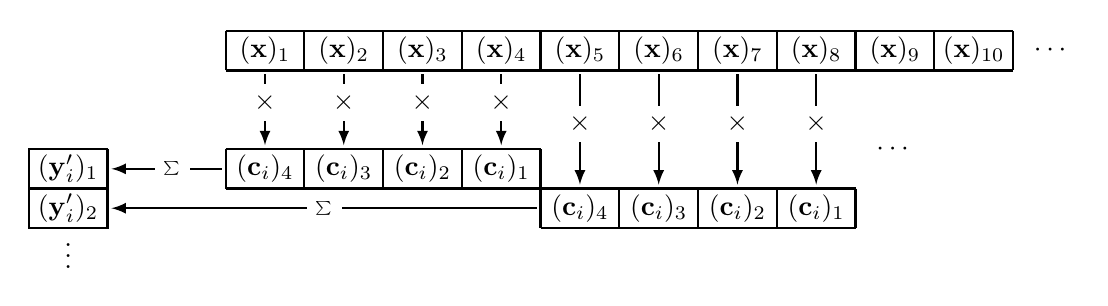
\begin{tikzpicture}
        \draw [black, thick] (-5,0.5) -- (5,0.5);
        \draw [black, thick] (-5,0) -- (5,0);

        \draw [black, thick] (-5,-1) -- (-1,-1);
        \draw [black, thick] (-5,-1.5) -- (-1,-1.5);
        \draw [black, thick] (-1,-1.5) -- (3,-1.5);
        \draw [black, thick] (-1,-2) -- (3,-2);
        \foreach \i in {-5,...,5} {
            \draw [black, thick] (\i, 0) -- (\i, 0.5);
        }
        \foreach \i in {1,...,10} {
            \draw ({\i-5.5},0.25) node[black] {$(\vec{x})_{\i}$};
        }

        \foreach \i in {-5,...,-1} {
            \draw [black, thick] (\i, -1) -- (\i, -1.5);
        }
        \foreach \i in {-5,...,-1} {
            \draw [black, thick] (\i+4, -1.5) -- (\i+4, -2);
        }
        
        \foreach \i in {4,...,1} {
            \draw ({(5-\i)-5.5},-1.25) node[black] {$(\vec{c}_i)_{\i}$};
        }
        \foreach \i in {4,...,1} {
            \draw ({(5-\i)-1.5},-1.75) node[black] {$(\vec{c}_i)_{\i}$};
        }
        \draw (3.5,-1) node[black] {$\cdots$};
        \draw (5.5,0.25) node[black] {$\cdots$};

        \foreach \i in {-5,...,-2} {
            \draw [black, thick, >=latex, ->] (\i+0.5,-0.05) -- node[pos=0.4,fill=white] {$\times$} (\i+0.5,-0.95);
        }
        \foreach \i in {-1,...,2} {
            \draw [black, thick, >=latex, ->] (\i+0.5,-0.05) -- node[pos=0.45,fill=white] {$\times$} (\i+0.5,-1.45);
        }
        \draw [black, thick, >=latex, ->] (-5.05,-1.25) -- node[pos=0.45,fill=white] {\tiny$\sum$} (-6.45,-1.25);
        \draw [black, thick, >=latex, ->] (-1.05,-1.75) -- node[pos=0.5,fill=white] {\tiny$\sum$} (-6.45,-1.75);
        \draw [black, thick] (-6.5,-1) -- (-6.5,-1.5) -- (-7.5,-1.5) -- (-7.5,-1) -- (-6.5,-1);
        \draw [black, thick] (-6.5,-1.5) -- (-6.5,-2) -- (-7.5,-2) -- (-7.5,-1.5) -- (-6.5,-1.5);
        \draw (-7,-1.25) node[black] {$(\vec{y}'_i)_1$};
        \draw (-7,-1.75) node[black] {$(\vec{y}'_i)_2$};
        \draw (-7,-2.25) node[black] {$\vdots$};
    \end{tikzpicture}
    \caption{Visualisation of $(\vec{y}_i)_1$ and $(\vec{y}_i)_2$ in the case that $N=4$}
    \label{fig:vis-yi}
\end{figure}

Consider the case that $\vec{c}_i = \begin{bmatrix}0 & 1 & 0 & 0\end{bmatrix}^T$. Then coset $i$ provides every second sample of all consecutive groups of four samples of the input signal. This is visualised in \cref{fig:vis-yi-case}.

\begin{figure}
    \centering
    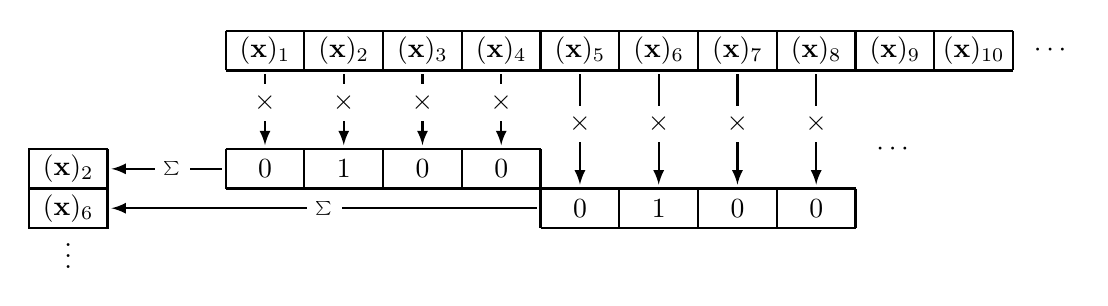
\begin{tikzpicture}
        \draw [black, thick] (-5,0.5) -- (5,0.5);
        \draw [black, thick] (-5,0) -- (5,0);

        \draw [black, thick] (-5,-1) -- (-1,-1);
        \draw [black, thick] (-5,-1.5) -- (-1,-1.5);
        \draw [black, thick] (-1,-1.5) -- (3,-1.5);
        \draw [black, thick] (-1,-2) -- (3,-2);
        \foreach \i in {-5,...,5} {
            \draw [black, thick] (\i, 0) -- (\i, 0.5);
        }
        \foreach \i in {1,...,10} {
            \draw ({\i-5.5},0.25) node[black] {$(\vec{x})_{\i}$};
        }

        \foreach \i in {-5,...,-1} {
            \draw [black, thick] (\i, -1) -- (\i, -1.5);
        }
        \foreach \i in {-5,...,-1} {
            \draw [black, thick] (\i+4, -1.5) -- (\i+4, -2);
        }
        
        \draw (-4.5,-1.25) node[black] {$0$};
        \draw (-3.5,-1.25) node[black] {$1$};
        \draw (-2.5,-1.25) node[black] {$0$};
        \draw (-1.5,-1.25) node[black] {$0$};
        \draw (-0.5,-1.75) node[black] {$0$};
        \draw (0.5,-1.75) node[black] {$1$};
        \draw (1.5,-1.75) node[black] {$0$};
        \draw (2.5,-1.75) node[black] {$0$};
        \draw (3.5,-1) node[black] {$\cdots$};
        \draw (5.5,0.25) node[black] {$\cdots$};

        \foreach \i in {-5,...,-2} {
            \draw [black, thick, >=latex, ->] (\i+0.5,-0.05) -- node[pos=0.4,fill=white] {$\times$} (\i+0.5,-0.95);
        }
        \foreach \i in {-1,...,2} {
            \draw [black, thick, >=latex, ->] (\i+0.5,-0.05) -- node[pos=0.45,fill=white] {$\times$} (\i+0.5,-1.45);
        }
        \draw [black, thick, >=latex, ->] (-5.05,-1.25) -- node[pos=0.45,fill=white] {\tiny$\sum$} (-6.45,-1.25);
        \draw [black, thick, >=latex, ->] (-1.05,-1.75) -- node[pos=0.5,fill=white] {\tiny$\sum$} (-6.45,-1.75);
        \draw [black, thick] (-6.5,-1) -- (-6.5,-1.5) -- (-7.5,-1.5) -- (-7.5,-1) -- (-6.5,-1);
        \draw [black, thick] (-6.5,-1.5) -- (-6.5,-2) -- (-7.5,-2) -- (-7.5,-1.5) -- (-6.5,-1.5);
        \draw (-7,-1.25) node[black] {$(\vec{x})_2$};
        \draw (-7,-1.75) node[black] {$(\vec{x})_6$};
        \draw (-7,-2.25) node[black] {$\vdots$};
    \end{tikzpicture}
    \caption{Visualisation of the case that $\vec{c}_i$ is chosen such that coset $i$ provides every second sample of all consecutive groups of four samples of the input signal}
    \label{fig:vis-yi-case}
\end{figure}

Let the correlation of the sampling vectors of cosets $i$ and $j$ be given by $\vec{r}_{c_i,c_j} = \vec{c}_i \circ \vec{c}_j$ and let the correlation of the pseudo outputs of cosets $i$ and $j$ be given by $\vec{r}_{y_i,y_j} = \vec{y}_i \circ \vec{y}_j$. Furthermore, let the correlation of the outputs of cosets $i$ and $j$ be given by $\vec{r}_{y'_i,y'_j} = \vec{y}'_i \circ \vec{y}'_j$. The goal of the reconstruction method is to reconstruct the autocorrelation of the input signal using the cross-correlations of the outputs of the cosets. We start by relating a subvector of $\vec{r}_{y'_i,y'_j}$ to a subvector of $\vec{r}_x$.

\begin{blockTheorem} \label{th:convolution-correlation}
    \makebox[\textwidth]{\centering $(\vec{c}_i \ast \vec{x}) \circ (\vec{c}_j \ast \vec{x}) = (\vec{c}_i \circ \vec{c}_j) \ast (\vec{x} \circ \vec{x})$.} \nolinebreak
\end{blockTheorem}

By \cref{th:convolution-correlation},
\begin{align*}
    \vec{r}_{y_i,y_j} =(\vec{c}_i \ast \vec{x}) \circ (\vec{c}_j \ast \vec{x}) = (\vec{c}_i \circ \vec{c}_j) \ast (\vec{x} \circ \vec{x}) = \vec{r}_{c_i,c_j} \ast \vec{r}_x.
\end{align*}
Denote a truncated version of $\vec{r}_{y_i,y_j}$ by
\begin{align*}
    \hat{\vec{r}}_{y_i,y_j} = \vec{r}_{y_i,y_j}[KLN-LN+2N-1,KLN+LN-1]
\end{align*}
and a truncated version of $\vec{r}_x$ by
\begin{align*}
    \hat{\vec{r}}_x = \vec{r}_x [KLN-LN+1,KLN+LN-1].
\end{align*}
Then
\begin{align*}
    \hat{\vec{r}}_{y_i,y_j}
    &= (\vec{r}_{c_i,c_j} \ast \vec{r}_x)[KLN-LN+2N-1,KLN+LN-1]\\
    &= (\vec{r}_x \ast \vec{r}_{c_i,c_j})[KLN-LN+2N-1,KLN+LN-1] \\
    &= \mat{R}_{c_i,c_j} \hat{\vec{r}}_x
\end{align*}
where $\mat{R}_{c_i,c_j}$ denotes the matrix
\begin{align*}
    \begin{bmatrix}
        % (\vec{r}_{c_i,c_j})_1 & 0 & 0& \cdots & 0 \\
        % (\vec{r}_{c_i,c_j})_2 & (\vec{r}_{c_i,c_j})_1 & 0 & \cdots & 0 \\
        % &  & \ddots &  & \\
        % 0 &  \cdots & 0 & (\vec{r}_{c_i,c_j})_{2N-1} & (\vec{r}_{c_i,c_j})_{2N-2} \\
        % 0 &  \cdots & 0& 0 & (\vec{r}_{c_i,c_j})_{2N - 1} \\
        (\vec{r}_{c_i,c_j})_{2N-1} & (\vec{r}_{c_i,c_j})_{2N-2} & \cdots &(\vec{r}_{c_i,c_j})_{1} & 0 & \cdots  \\
        0 & (\vec{r}_{c_i,c_j})_{2N-1} & \cdots & (\vec{r}_{c_i,c_j})_{2} & (\vec{r}_{c_i,c_j})_{1} & \cdots \\
        && \multicolumn{2}{c}{\ddots} \\
        \cdots & (\vec{r}_{c_i,c_j})_{2N-1} & (\vec{r}_{c_i,c_j})_{2N-2} & \cdots & (\vec{r}_{c_i,c_j})_{1} & 0 \\
        \cdots & 0 & (\vec{r}_{c_i,c_j})_{2N-1} & \cdots &(\vec{r}_{c_i,c_j})_{2} & (\vec{r}_{c_i,c_j})_{1} 
    \end{bmatrix}.
\end{align*}

Since we have related $\hat{\vec{r}}_{y_i,y_j}$ to $\hat{\vec{r}}_x$, we now make effort to relate a subvector of $\vec{r}_{y'_i,y'_j}$ to $\hat{\vec{r}}_{y_i,y_j}$. To this end, let the $2L-1\times 2LN-2N+1$ decimation matrix be defined by $(\mat{D})_{i,(i-1)N+1} = 1$ for $i=1,\ldots,2L-1$ and otherwise zero. Let the decimated truncated correlation of the pseudo outputs of cosets $i$ and $j$ be given by $\hat{\vec{r}}'_{y_i,y_j} = \mat{D} \hat{\vec{r}}_{y_i,y_j}$. Denote a truncated version of $\vec{r}_{y'_i,y'_j}$ by $\hat{\vec{r}}_{y'_i,y'_j}=\vec{r}_{y'_i,y'_j}[KL-L+1,KL+L-1]$. The following theorem relates $\hat{\vec{r}}_{y'_i,y'_j}$ to $\hat{\vec{r}}'_{y_i,y_j}$.

\begin{blockTheorem} \lab{th:deci-corr}
    Let $Y_i[n]$ and $Y_j[n]$ be wide sense stationary stochastic processes such that $(\vec{y}_i)_m = Y_i[m]$ and $(\vec{y}_j)_m = Y_j[m]$ for $m=1,\ldots,KLN+N-1$. Furthermore, let $Y'_i[n]$ and $Y'_j[n]$ be wide sense stationary stochastic processes such that $(\vec{y}'_i)_m = Y'_i[m]$ and $(\vec{y}'_j)_m = Y'_j[m]$ for $m=1,\ldots,KL$. Then $N\hat{\vec{r}}_{y'_i,y'_j}$ is an unbiased estimator of $\vec{w} \odot E(\hat{\vec{r}}'_{y_i,y_j})$ where

    \makebox[\textwidth]{\centering
        $\vec{w} = \begin{bmatrix}
            KLN+(-L+2)N-1 \\
            KLN+(-L+3)N-1 \\
            \vdots \\
            KLN+0\cdot N-1 \\
            KLN+1\cdot N-1 \\
            KLN+0\cdot N-1 \\
            \vdots \\
            KLN+(-L+3)N-1 \\
            KLN+(-L+2)N-1
         \end{bmatrix} \odot \begin{bmatrix}
            [KLN+(-L+1)N]^{-1} \\
            [KLN+(-L+2)N]^{-1} \\
            \vdots \\
            (KLN -1 \cdot N)^{-1} \\
            (KLN+ 0 \cdot N)^{-1} \\
            (KLN -1 \cdot N)^{-1} \\
            \vdots \\
            [KLN+(-L+2)N]^{-1} \\
            [KLN+(-L+1)N]^{-1}
         \end{bmatrix}.$
    }
\end{blockTheorem}

Finally, we relate $\hat{\vec{r}}_x$ to the autocorrelation of the input signal and $\hat{\vec{r}}_{y'_i,y'_j}$ to the cross-correlation of the outputs of cosets $i$ and $j$. To do this, we identify the expected value of $\hat{\vec{r}}_x$ and $\hat{\vec{r}}_{y'_i,y'_j}$.

Let $X[n]$ be a wide sense stationary stochastic process such that $(\vec{x})_i = X[i]$ for $i = 1,\ldots,KLN$. Also, let $\vecsc{r}_x \in \mathbb{C}^{2LN-1}$ be such that $(\vecsc{r}_x)_{i+LN} = R_X[i]$ for $i = -LN + 1, LN-1$ and let $\vecsc{r}_{y'_i,y'_j} \in \mathbb{C}^{2L-1}$ be such that $(\vecsc{r}_{y'_i,y'_j})_{i+L}=R_{Y'_i,Y'_j}[i]$ for $i = -L+1,L-1$.
Note that $\vecsc{r}_x$ represents the unbiased autocorrelation of the input signal and that $\vecsc{r}_{y'_i,y'_j}$ represents the unbiased crosscorrelation of the outputs of cosets $i$ and $j$. Then by \cref{th:correlation-bias}, $E(\hat{\vec{r}}_x) = \vec{b}_x \odot \vecsc{r}_x$ and $E(\hat{\vec{r}}_{y'_i,y'_j})=\vec{b}_{y'} \odot \vecsc{r}_{y'_i,y'_j}$ where
\begin{align*}
    \vec{b}_{x} =  \begin{bmatrix}
        (K-1)LN+1 \\
        (K-1)LN+2 \\
        \vdots \\
        KLN \\
        \vdots \\
        (K-1)LN+2 \\
        (K-1)LN+1
    \end{bmatrix},\vec{b}_{y'} = \begin{bmatrix}
        (K-1)L + 1 \\
        (K-1)L + 2 \\
        \vdots \\
        KL \\
        \vdots \\
        (K-1)L + 2 \\
        (K-1)L + 1
    \end{bmatrix}.
\end{align*}

% Then
% \begin{align*}
%     E(\hat{\vec{r}}'_y) &= \begin{bmatrix}
%         E(N\hat{\vec{r}}_{y'_1,y'_1}) \\
%         \vdots \\
%         E(N\hat{\vec{r}}_{y'_M,y'_M})
%     \end{bmatrix} \\
%     &= \begin{bmatrix}
%         N\vec{b}_y \odot \vec{r}_{y'_1,y'_1,u} \\
%         \vdots \\
%         N\vec{b}_y \odot \vec{r}_{y'_M,y'_j,M}
%     \end{bmatrix} \\
%     &= \begin{bmatrix} 
%         \vec{w} \odot E(\hat{\vec{r}}'_{y_1,y_1}) \\
%         \vdots \\
%         \vec{w} \odot E(\hat{\vec{r}}'_{y_M,y_M}) \\
%     \end{bmatrix} \\
%     &= \begin{bmatrix}
%         \vec{w} \odot \mat{D}\mat{R}_{c_1,c_1} E(\hat{\vec{r}}_x) \\
%         \vdots \\
%         \vec{w} \odot \mat{D}\mat{R}_{c_M,c_M} E(\hat{\vec{r}}_x) \\
%     \end{bmatrix} \\
%     &= \begin{bmatrix}
%         \vec{w} \odot \mat{D}\mat{R}_{c_1,c_1} (\vec{b}_x \odot \vec{r}_{x,u}) \\
%         \vdots \\
%         \vec{w} \odot \mat{D}\mat{R}_{c_M,c_M} (\vec{b}_x \odot \vec{r}_{x,u}) \\
%     \end{bmatrix}.
%     % = E\left(\begin{bmatrix}
%     %     \vec{w} \odot \vec{r}'_{y_1,y_1} \\
%     %     \vdots \\
%     %     \vec{w} \odot \vec{r}'_{y_M,y_M} \\
%     % \end{bmatrix}\right) = E(\mat{R} \hat{\vec{r}}_x) = \mat{R} E(\hat{\vec{r}}_x).
% \end{align*}
Now $E(N\hat{\vec{r}}_{y'_i,y'_i}) = N\vec{b}_{y'} \odot \vecsc{r}_{y'_i,y'_i}$, whilst also
\begin{align*}
    E(N\hat{\vec{r}}_{y'_i,y'_i}) = \vec{w} \odot E(\hat{\vec{r}}'_{y_i,y_i}) = \vec{w} \odot \mat{D}\mat{R}_{c_i,c_j} E(\hat{\vec{r}}_x) = \vec{w} \odot \mat{D}\mat{R}_{c_i,c_i} (\vec{b}_x \odot \vecsc{r}_{x}).
\end{align*}
Therefore equating and dividing by $KLN$ yields that
\begin{align*} 
    \left(\frac{\vec{b}_{y'}}{KL}\right) \odot \vecsc{r}_{y'_i,y'_j} = \vec{w} \odot \mat{D}\mat{R}_{c_i,c_i} \left[\left(\frac{\vec{b}_x}{KLN}\right) \odot \vecsc{r}_{x}\right],
\end{align*}
or equivalently
\begin{align} \label{eq:bias-relationship}
    \vecsc{b}_{y'} \odot \vecsc{r}_{y'_i,y'_j} = \mat{D} \mat{R}_{c_i,c_j} (\vecsc{b}_x \odot \vecsc{r}_x)
\end{align}
where $(\vecsc{b}_x)_i = (\vec{b}_x)_i/KLN$ for $i = 1,\ldots,2LN-1$ and $(\vecsc{b}_{y'})_i = (\vec{b}_{y'})_i/[KL (\vec{w})_i]$ for $i = 1,\ldots,2L-1$. This equation relates the autocorrelation of the input signal to the cross-correlation of the outputs of cosets $i$ and $j$. However, this relationship involves element-wise multiplication, which shows that a biased estimate of $\vecsc{r}_{y'_i,y'_j}$ is related to a biased estimate of $\vecsc{r}_x$.

TODO: visualisation of biases

% \begin{figure}[H]
%     \centering
%     \begin{tikzpicture}
%         \draw [thick,black] (-5,0) -- (5,0);
%         \draw [thick,black] (-5,-0.1) -- (-5,0.1);
%         \draw [thick,black] (5,-0.1) -- (5,0.1);
%         \draw [thick,black] (0,-0.1) -- (0,0.1);
%         \draw [thick,black] (-3,0.1) -- (-3,-0.1);
%         \draw [thick,black] (3,-0.1) -- (3,0.1);
%         \draw [dashed] (-5,0.6) -- (5,0.6);
%         \draw [black,thick] (-5,0) -- (0,1.5) -- (5,0);
%         \draw [dashed] (-5,1.5) -- (5,1.5);
%         \draw (6,1.5) node[black] {$1$};
%         \draw (6,0.6) node[black] {$\frac{(K-1)LN+1}{KLN}$};
%         \draw (-3,-0.4) node[black] {$(\vecsc{b}_x)_1$};
%         \draw (0,-0.4) node[black] {$(\vecsc{b}_x)_{LN}$};
%         \draw (3,-0.4) node[black] {$(\vecsc{b}_x)_{2LN-1}$};
%         \draw (-1.5,0) node[black,fill=white] {$\cdots$};
%         \draw (1.5,0) node[black,fill=white] {$\cdots$};
%     \end{tikzpicture}
%     \caption{Visualisation of $\vecsc{b}_x$}
%     \label{fig:vis-bx}
% \end{figure}

% \begin{figure}[H]
%     \centering
%     \begin{tikzpicture}
%         \draw [thick,black] (-5,0) -- (5,0);
%         \draw [thick,black] (-5,-0.1) -- (-5,0.1);
%         \draw [thick,black] (5,-0.1) -- (5,0.1);
%         \draw [thick,black] (0,-0.1) -- (0,0.1);
%         \draw [thick,black] (-3,0.1) -- (-3,-0.1);
%         \draw [thick,black] (3,-0.1) -- (3,0.1);
%         \draw [dashed] (-5,0.6) -- (5,0.6);
%         \draw [black,thick] (-5,0) -- (0,1.5) -- (5,0);
%         \draw [dashed] (-5,1.5) -- (5,1.5);
%         \draw (7.5,1.5) node[black] {$\frac{KLN}{KLN+N-1}$};
%         \draw (7.5,0.6) node[black] {$\frac{[(K-1)L+1][KLN+(-L+1)N]}{KL[KLN+(-L+2)N-1]}$};
%         \draw (-3,-0.4) node[black] {$(\vecsc{b}_y)_1$};
%         \draw (0,-0.4) node[black] {$(\vecsc{b}_y)_{L}$};
%         \draw (3,-0.4) node[black] {$(\vecsc{b}_y)_{2L-1}$};
%         \draw (-1.5,0) node[black,fill=white] {$\cdots$};
%         \draw (1.5,0) node[black,fill=white] {$\cdots$};
%     \end{tikzpicture}
%     \caption{Visualisation of $\vecsc{b}_{y'}$}
%     \label{fig:vis-by}
% \end{figure}
We now aggregate \cref{eq:bias-relationship} for all combinations of cosets. Let $\vecsc{b}_y$, $\vecsc{r}_y$ and $\vec{R}$ be such that
\begin{align}
    \begin{bmatrix}
        \vecsc{b}_{y'} \odot \vecsc{r}_{y'_1,y'_1} \\ \vdots \\ \vecsc{b}_{y'} \odot \vecsc{r}_{y'_M,y'_M}
    \end{bmatrix} &= \begin{bmatrix}
        \vecsc{b}_{y'} \\ \vdots \\ \vecsc{b}_{y'}
    \end{bmatrix} \odot \begin{bmatrix}
        \vecsc{r}_{y'_1,y'_1} \\ \vdots \\ \vecsc{r}_{y'_M,y'_M}
    \end{bmatrix} \nonumber \\
    &= \vecsc{b}_y \odot \vecsc{r}_y \nonumber \\
    &= \begin{bmatrix}
        \mat{D}\mat{R}_{c_1,c_1} \\ \vdots \\ \mat{D}\mat{R}_{c_M,c_M}
    \end{bmatrix} (\vecsc{b}_x \odot \vecsc{r}_x) \nonumber \\
    &= \mat{R} (\vecsc{b}_x \odot \vecsc{r}_x). \label{eq:relationship-biased-aggregated}
\end{align}
It is important to notice that $\mat{R}$ in an $M^2(2L-1)\times 2LN-1$ matrix. This means that the relationship may be invertible, which dependens on whether $\mat{R}$ has full column rank.


\subsection{Limiting Process}
It is important to notice that in \cref{eq:relationship-biased-aggregated} only $\vecsc{b}_x$ and $\vecsc{b}_y$ depend on $K$. This is remarkable, since this implies that $\mat{R}$ can be used to relate the estimates of $\vecsc{r}_x$ and $\vecsc{r}_{y}$ biased by $\vecsc{b}_x$ and $\vecsc{b}_y$ for any $K$. Furthermore, this means that the relationship still holds when $K \to \infty$. If $K \to \infty$, then $\vecsc{b}_x \to \vec{1}_{2LN-1}$ and $\vecsc{b}_y \to \vec{1}_{2L-1}$. Therefore, we see that
\begin{align*}
    \vecsc{b}_y \odot \vecsc{r}_{y} \to \vec{1}_{2L-1}\odot \vecsc{r}_{y} = \vecsc{r}_{y}
\end{align*}
and
\begin{align*}
    \mat{R} (\vecsc{b}_x \odot \vecsc{r}_x)\to \mat{R} (\vec{1}_{2LN-1} \odot \vecsc{r}_x) = \mat{R} \vecsc{r}_x.
\end{align*}
Therefore
\begin{align} \label{eq:relationship-unbiased}
    \vecsc{r}_{y} = \mat{R} \vecsc{r}_{x}.
\end{align}
% The limit $\vecsc{b}_x \to \vec{1}_{2LN-1}$ when $K \to \infty$ is depicted (..).
% \begin{figure}[H]
%     \centering
%     \begin{tikzpicture}
%         \draw [thick,black] (-5,0) -- (5,0);
%         \draw [thick,black] (-5,-0.1) -- (-5,0.1);
%         \draw [thick,black] (5,-0.1) -- (5,0.1);
%         \draw [thick,black] (0,-0.1) -- (0,0.1);
%         \draw [thick,black] (-3,0.1) -- (-3,-0.1);
%         \draw [thick,black] (3,-0.1) -- (3,0.1);
%         \draw [dashed] (-6,0.6) -- (6,0.6);
%         \draw [black,thick] (-5,0) -- (0,1.5) -- (5,0);
%         \draw [red,thick] (-6,1.5) -- (6,1.5);
%         \draw (7,1.5) node[black] {$1$};
%         \draw (7,0.6) node[black] {$\frac{(K-1)LN+1}{KLN}$};
%         \draw (-3,-0.4) node[black] {$(\vecsc{b}_x)_1$};
%         \draw (0,-0.4) node[black] {$(\vecsc{b}_x)_{LN}$};
%         \draw (3,-0.4) node[black] {$(\vecsc{b}_x)_{2LN-1}$};
%         \draw (-1.5,0) node[black,fill=white] {$\cdots$};
%         \draw (1.5,0) node[black,fill=white] {$\cdots$};
%         \draw [fill=red,red] (-3,0.6) circle[radius=0.05];
%         \draw [fill=red,red] (-3,1.5) circle[radius=0.05];
%         \draw [fill=red,red] (3,0.6) circle[radius=0.05];
%         \draw [fill=red,red] (3,1.5) circle[radius=0.05];
%         \draw [fill=red,red] (5,0) circle[radius=0.05];
%         \draw [fill=red,red] (-5,0) circle[radius=0.05];
%         \draw [thick,red,>=latex,->] (-3,0.6) -- (-3,1.5);
%         \draw [thick,red,>=latex,->] (3,0.6) -- (3,1.5);
%         \draw [thick,red,>=latex,->] (5,0) -- (6,0);
%         \draw [thick,red,>=latex,->] (-5,0) -- (-6,0);
%         \draw [red] (-6.3,0) node[red] {$\infty$};
%         \draw [red] (6.3,0) node[red] {$\infty$};
%         \draw (0,2) node[red] {$K \to \infty$};
%     \end{tikzpicture}
%     \caption{Visualisation of $\vecsc{b}_x \to \vec{1}_{2LN-1}$ when $K \to \infty$. The red line depicts the limit.}
%     \label{fig:vis-bx}
% \end{figure}



\subsection{Limiting Support}
It is often assumed that $R_{Y'_i,Y'_j}$ is limited in support. This assumption turns out to be helpful later on. Therefore, assume that $R_{Y'_i,Y'_j}[m] = 0$ for 
\begin{align*}
     -KL+1 \le m \le -L \text{ and } L \le m \le KL-1.
\end{align*}
The proof of \cref{th:convolution-correlation} then shows that $R_{Y_i,Y_j}[m]=0$ for 
\begin{align*}
    -KLN+N \le m \le -LN \text{ and } LN \le m \le KLN-N,
\end{align*}
which implies that $[E(\vec{r}_{y_i,y_j})]_{m}=0 $ for 
\begin{align*}
    2N-1 \le m \le KLN - LN + N - 1
\end{align*}
and
\begin{align*}
    KLN +LN + N - 1 \le m \le 2KLN -1.
\end{align*}
Since $\vec{r}_{y_i,y_j} = \vec{r}_{c} \ast \vec{r}_x$, $[E(\vec{r}_x)]_m=0$ for 
\begin{align*}
    1 \le m \le KLN - LN + N - 1 \text{ and } KLN + LN - N + 1 \le m \le 2KLN - 1,
\end{align*}
which yields that $R_X[m]=0$ for 
\begin{align*}
    -KLN + 1\le m \le -LN+N-1 \text{ and } LN-N+1 \le m \le KLN - 1.
\end{align*}
Therefore $(\vecsc{r}_x)_m = 0$ for 
\begin{align*}
    1 \le m \le N-1 \text{ and } 2LN-N+1 \le 2LN-1.
\end{align*}
The limited support of $\vecsc{r}_x$ now yields that
\begin{align} \label{eq:unbiased-relationship}
    \vecsc{b}_y \odot \vecsc{r}_y &= \mat{R}[N,2LN-N] (\vecsc{b}_x \odot \vecsc{r}_x)[N,2LN-N], \\
    \vecsc{b}_y &= \mat{R}[N,2LN-N] \vecsc{r}_x[N,2LN-N].
\end{align}
These equations conclude the main analysis.


% So $\vec{r}_y'$ is an unbiased estimator of $\mat{R} E(\hat{\vec{r}}_x)$, which we can use to determine $E(\hat{\vec{r}}_x)$. Denote $\vec{x}_m = \vec{x}[(m-1)N+1,mN]$ for $m = 1,\ldots,L$. Thus $\vec{x}_m$ corresponds to the $m$'th interval of $N$ samples of $\vec{x}$. Finally, note that
% \begin{align*}
%     (\vec{y}'_i)_m = (\vec{y}_i)_{mN} = (\vec{c}_i \ast \vec{x})_{mN} = \sum_{k=1}^N (\vec{c}_i)_k (\vec{x})_{mN - k + 1} = \vec{d}_i \cdot \vec{x}_m
% \end{align*}
% where $\vec{d}_i$ denotes $\vec{c}_i$ reversed. Therefore, the reverse of the sampling vector for a coset determines the output of the coset for every interval of $N$ samples of $\vec{x}$. Accordingly, let
% \begin{align*}
%     \vec{w}_m = \begin{bmatrix}
%         (\vec{y}'_1)_m \\
%         \vdots \\
%         (\vec{y}'_M)_m
%     \end{bmatrix} = \begin{bmatrix}
%         \vec{d}_1 \cdot \vec{x}_m \\
%         \vdots \\
%         \vec{d}_M \cdot \vec{x}_m
%     \end{bmatrix} = \begin{bmatrix}
%         \vec{d}_1^T\\
%         \vdots \\
%         \vec{d}_M^T
%     \end{bmatrix} \vec{x}_m.
% \end{align*}
% Thus $\vec{w}_m$ aggregates the output of all cosets in the $m$'th interval of $N$ samples of $\vec{x}$. This concludes the main analysis.


\end{document}